\subsubsection{Graphs}

As with the scheduler, the implementation of the graphs has been divided between model, controller, and view components.

\subsubsection{Graphs Model}

The model has the simple task of storing the logged data, and providing the dataset upon request.

\begin{figure}[H]
\centering{}
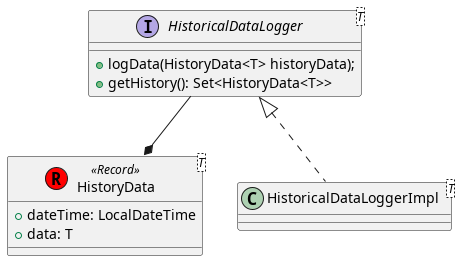
\includegraphics[width=\textwidth,height=\textheight,keepaspectratio]{magnani/uml/graph-model.png}
\caption{UML diagram of the graph model}
\label{magnani:uml:graph-model}
\end{figure}

\subsubsection{Graphs Controller}

The controller has the task of supplying the data to log to the model, and to refresh the view.
It has been generalized with the use of a \texttt{Supplier} in an abstract implementation \texttt{AbstractLogger}. \newline
The supplier decides how to retrieve the data to log, effectively becoming an abstract method, and the updateTick (where the data is logged)
becomes a template method.

\begin{figure}[H]
\centering{}
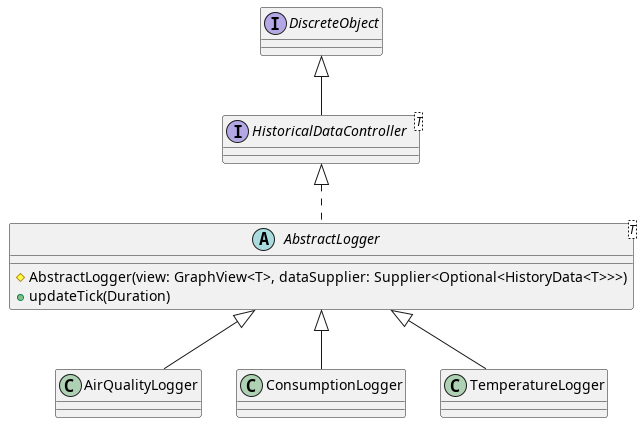
\includegraphics[width=\textwidth,height=\textheight,keepaspectratio]{magnani/uml/graph-controller.png}
\caption{UML diagram of the graph controller}
\label{magnani:uml:graph-controller}
\end{figure}

\paragraph{Problem} We have to choose which thermometer to log.
\paragraph{Solution} Use the first/any thermometer found.
This solution would not work with multiple thermometers in different environments.
In that case it would be better to choose a particular thermometer to log, and/or to have multiple logs for all the different thermometers.

\paragraph{Problem} We have to choose how to log the data.
\paragraph{Solution} I chose to log the data at each (simulation) hour for design simplicity.
Could also have logged each tick, but it would have led to some pretty confusing graphs if the time rate were to be modified
due to the time axis not being linear.
In the future, the time between each log could be configured.
It could also be possible to log more frequently but choose to display at a larger interval of time.

\subsubsection{Graphs View}

The graph view has the task of displaying the historical data, sent from the controller, to the user.

\begin{figure}[H]
\centering{}
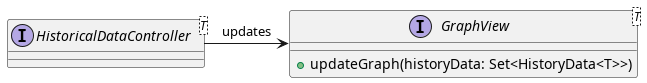
\includegraphics[width=\textwidth,height=\textheight,keepaspectratio]{magnani/uml/graph-view.png}
\caption{UML diagram of the graph view}
\label{magnani:uml:graph-view}
\end{figure}

\paragraph{Problem} How to handle the display of the new data.
\paragraph{Solution} I chose to refresh all the data each update for design simplicity.
Another way would have been to send only the new data from the graph controller to the view,
this would have required the view to decide whether to discard the oldest data record,
and due to time constraints, I just decided to go with the simplest way.
It also allowed me to better separate the logic and view, in fact it's the controller
deciding what to display.
